\documentclass[11pt]{article}

\usepackage[utf8]{inputenc}
\usepackage[T1]{fontenc}
\usepackage{lmodern}
\usepackage[a4paper, margin=2.5cm]{geometry}
\usepackage{graphicx}
\usepackage{booktabs}
\usepackage{caption}
\usepackage{subcaption}
\usepackage{amsmath}
\usepackage{hyperref}
\usepackage{authblk}
\usepackage[round]{natbib}
\usepackage{setspace}
\onehalfspacing
\graphicspath{{figures/}}

\title{Statistical structure of natural images and individual creativity\\
       jointly shape visual pareidolia}

\author{[Authors]}
\date{Draft \today}

\begin{document}
\maketitle

\begin{abstract}
\noindent
Pareidolia, the perception of meaningful figures in noise, is one
of the most accessible everyday demonstrations of top-down vision, yet
has rarely been studied at a scale that resolves both the contribution
of the image and that of the observer. We collected $N \approx 580$
online sessions in which participants viewed 30 fractal-noise patches
spanning three controlled fractal-dimension levels (FD12, FD14, FD16)
and freely typed every percept that came to mind, before and after
completing the Divergent Association Task (DAT,
\citealp{Olson2021dat}) as a stable measure of trait creativity. A
subset opted in to webcam-based eye tracking. Across 18{,}500 unique
percept reports we show (\emph{i}) that the statistical complexity of
the image (FD) systematically reshapes both \emph{what} people see, 
shifting the modal percept from anthropomorphic figures at low
complexity to animals at intermediate complexity to textural
descriptions at high complexity, and \emph{how} they explore the
image; (\emph{ii}) that trait creativity predicts a small but reliable
bias toward animal-like and away from human-like percepts, higher
semantic diversity at intermediate complexity, and a measurable
preference for specific embodied or unusual categories;
and (\emph{iii}) that DAT scores measured immediately after the
pareidolia task remain strongly correlated with the baseline score but
no longer predict the same behavioural patterns, consistent with the
DAT, pareidolia association capturing a trait-level property of the
observer rather than a transient state shift induced by the task.
\end{abstract}

%==============================================================
\section{Methods}
%==============================================================

\subsection{Participants and recruitment}
Participants were recruited online via [recruitment platform]; all gave
informed consent in accordance with the [ethics committee] guidelines.
The full session was completed by $N = 579$ English-speaking adults
(the ``main cohort''), comprising a demographic form, the 10-word
Divergent Association Task \citep{Olson2021dat} as a baseline measure
of trait creativity (DAT-pre), an optional 9-point WebGazer calibration
and validation routine, 30 pareidolia trials with free-response word
entry, a repeated DAT (DAT-post; $n = 507$ provided a scoreable
response), and a closing feedback questionnaire. The main cohort
analysed below is defined as the intersection of (\emph{i}) English
primary language, (\emph{ii}) feedback supplied, and (\emph{iii}) at
least one valid pareidolia trial. Sessions whose stored DAT word list
duplicated one of the previous two log entries (an artefact of repeat
submission) were removed.

\subsection{Stimuli}
The stimulus set comprised 30 grey-scale fractal-noise images, ten at
each of three fractal-dimension levels (\textbf{FD12}, \textbf{FD14},
\textbf{FD16}; FD~$\in \{1.2, 1.4, 1.6\}$ in the 2-D plane). FD was
controlled by the slope of the amplitude spectrum prior to inverse
Fourier transform, with higher FD producing finer-grained spatial
detail and lower local autocorrelation. Each participant saw all 30
images in a fully randomised order. Each image was rendered centred on
a white viewport with \texttt{max-width: 55\%} (jsPsych
\texttt{image-keyboard-response}), preserving the image's aspect ratio.

\subsection{Procedure per trial}
A pareidolia trial began with a 500-ms central fixation cross, followed
by the stimulus image presented for up to 30~s, terminated early if the
participant pressed the spacebar to advance. Immediately after stimulus
offset a free-text response screen appeared with five short-answer
slots labelled ``Single words'' and five longer slots labelled
``Descriptions (optional)''; participants were instructed to write
every distinct percept that the image evoked. When eye tracking had
been enabled at session start, raw $(x, y, t)$ gaze samples were
captured throughout image presentation via the WebGazer browser-side
extension to jsPsych.

\subsection{Percept-word pre-processing}
Each typed entry was lowercased and whitespace-stripped. To minimise
contamination by non-percept entries we kept only entries matching the
regular expression \verb|^[A-Za-z]+$| (i.e., single alphabetic tokens
without spaces, digits, or punctuation), and additionally removed the
catch-all stop-words \emph{nothing, nothingness, black, white, map,
cloud, clouds}. Sentence-level descriptions were excluded from semantic
analyses to avoid mixing single-word and multi-word vector
representations, which occupy systematically different regions of the
embedding space. All semantic computations use 384-dimensional
sentence-transformer embeddings (\texttt{all-MiniLM-L6-v2}) of every
unique surviving percept word ($n_{\text{words}} = 4{,}361$).

\subsection{DAT scoring}
Both DAT-pre and DAT-post were scored with the canonical
\citet{Olson2021dat} procedure. Each set of 10 candidate words was
lowercased and restricted to alphabetic forms; the first seven words
with a GloVe~840B 300-d vector were retained, and the DAT score was
defined as $100 \cdot \text{mean}(d_{ij})$, where $d_{ij}$ is the
cosine distance between every pair of those seven vectors. Sessions
producing fewer than seven valid lookups yielded no DAT score and were
excluded from any analysis using that timepoint. DAT scores in
main-text analyses refer to the baseline (\emph{pre}) score unless
explicitly noted; analyses using the post-task score are reported in
the section on creativity (\ref{sec:dat}).

\subsection{Eye-tracking pre-processing}
The on-line WebGazer calibration sweep provides a dense set of gaze
samples spanning most of the viewport. For each session, we estimated
the usable gaze extent as the 1st-to-99th-percentile box of these
calibration samples and used it to rescale all subsequent gaze data
into the unit square $[0, 1]$, eliminating cross-session differences
in screen size and browser viewport. The stimulus region of interest
(ROI) was approximated as a per-session rectangle centred on the
recorded stimulus position with half-width $0.275$ (\(=\) half of the
\texttt{55\%} CSS rule) and half-height $0.275 \cdot W/H$, where
$W/H$ is the session's viewport aspect ratio. Trials whose normalised
gaze trace formed a near-perfect line, defined as
$|\text{corr}(x, y)| > 0.97$ together with span $> 0.6$ on both axes,
a signature of the WebGazer face-mesh tracker failing onto a screen
edge, were flagged as tracking failures and dropped (530 of 5{,}660
trials, 9.4\%). Fixations were detected with a dispersion-threshold
(I-DT) algorithm using a dispersion bound of $0.05$ in normalised
coordinates and a minimum duration of 100~ms. Eye-tracking analyses
are restricted to the 247 participants for whom at least one trial
survived these filters.

\subsection{Per-participant and per-image semantic metrics}
For every participant and every FD level we computed (\emph{i}) the
\emph{semantic spread} of percepts as the median pair-wise cosine
distance over their unique word embeddings, and (\emph{ii}) the
\emph{vocabulary surprisal} as the mean $-\log p$ over the corpus
frequency of each word. To examine the \emph{kind} of percept rather
than its amount, we assigned every unique word to one of fourteen
semantic categories (\emph{face, body-part, person, mammal, bird,
fish-aquatic, insect-bug, creature, object, landscape, weather,
abstract, food, tool}) by nearest seed-centroid in BERT space
(minimum cosine $\geq 0.30$, otherwise ``other''). For each
(participant, FD) we summarised the percept distribution as the
\emph{human share} (face $+$ body-part $+$ person), the
\emph{animal share} (mammal $+$ bird $+$ fish $+$ insect), and the
\emph{animal, human bias index} $(A - H) / (A + H)$, ranging from
$-1$ (entirely human) to $+1$ (entirely animal). At the image level
we computed the Shannon entropy of the percept-word distribution
elicited by each stimulus, as a measure of inter-observer consensus.

\subsection{Data-driven percept clustering}
To complement the seed-based taxonomy with an unsupervised view, we
clustered every percept word that appeared at least three times in the
corpus ($n = 1{,}110$ words). The BERT embeddings were
L2-normalised, reduced to 10 dimensions with UMAP (cosine metric,
\texttt{n\_neighbors}~=~15, \texttt{min\_dist}~=~0), and clustered
with HDBSCAN (\texttt{min\_cluster\_size}~=~12,
\texttt{cluster\_selection\_method}~=~\textsc{eom}). The procedure
produced 32 interpretable clusters plus a noise group (22\% of words).
Each cluster was labelled by its top four log-odds most distinctive
words, i.e., the words whose probability inside the cluster most
exceeds their probability outside it.

\subsection{Statistical analyses}
Within-subject effects of FD were tested with Friedman's $\chi^2$
followed by pair-wise Wilcoxon signed-rank contrasts; only contrasts
significant at $p < 0.05$ are annotated on the figures (brackets with
asterisks). Between-subject DAT effects were tested with Pearson's $r$
(reported in the main figures) and Spearman's $\rho$ (reported in the
companion CSV tables). Before every correlation we trimmed bivariate
outliers at $\pm 3$~SD on both the dependent metric and the DAT score;
no other transformations were applied. For the cluster-preference
forest plot, 95\% bootstrap CIs (2{,}000 binomial resamples per
cluster) were computed on the log-odds of the (High~/~Low) tertile
share. Statistics are reported as $r$ with significance marker
($^*p<0.05,\,^{**}p<0.01,\,^{***}p<0.001$); exact $p$ values and the
Spearman counterparts are given in the supplementary data tables. All
analyses were performed in Python 3.10 using
\texttt{pandas}, \texttt{numpy}, \texttt{scipy.stats},
\texttt{sentence-transformers}, \texttt{umap-learn} and
\texttt{hdbscan}; reproducible scripts and CSV outputs are available
at [URL].

%==============================================================
\section{Results}
%==============================================================

%, , , , , , , , , , , , , , , , , , , ,, 
\subsection{Stimulus complexity shapes the amount of pareidolia}
%, , , , , , , , , , , , , , , , , , , ,, 

We first asked whether the image's statistical structure itself
modulates how readily participants extract a percept. As image
complexity rose from FD12 to FD16, the average number of single words
submitted per trial decreased monotonically from $1.69$ to $1.56$
(Friedman $\chi^2 = 46.5$, $p = 7.9 \times 10^{-11}$;
Fig.~\ref{fig:fd_behaviour}), and the parallel decrease in the number
of free-text descriptions per trial was equally robust (Friedman
$p = 6.7 \times 10^{-10}$). The within-subject median semantic spread
of percepts at each FD, a participant-level index of how
semantically scattered their answers were on the stimuli of a given
complexity, decreased slightly but reliably with FD (Friedman
$p = 0.02$). Mean reaction time did not differ by FD (Friedman
$p = 0.17$). Together, these results suggest that as the image
becomes less locally autocorrelated, fewer recognisable shapes survive
the perceptual interpretation, both in absolute count and in semantic
diversity. They establish FD as a manipulation that biases observers
toward fewer, and progressively more uniform, percepts.

\begin{figure}[ht]
\centering
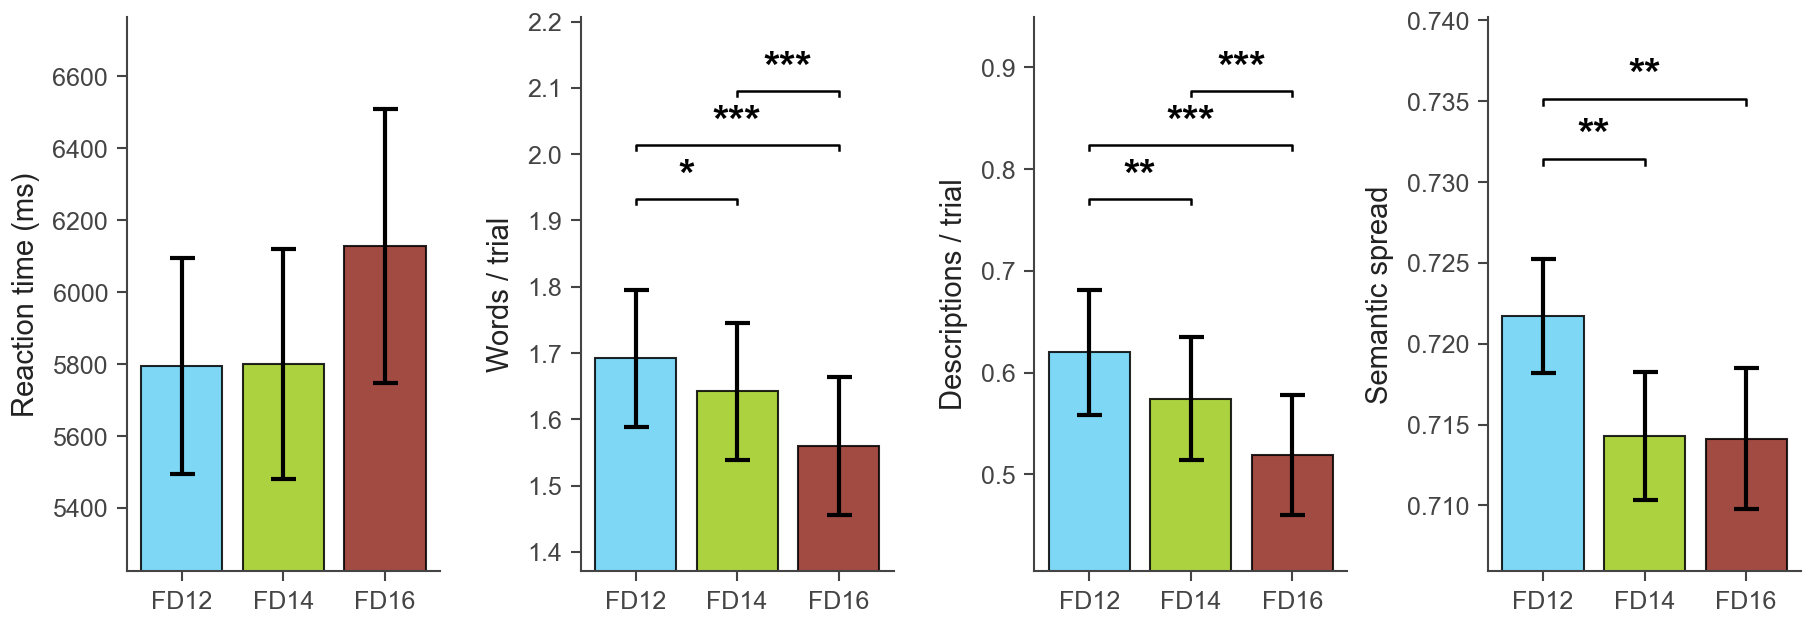
\includegraphics[width=\linewidth]{fig1_fd_behaviour.png}
\caption{\textbf{Stimulus FD shapes behavioural pareidolia.}
Within-subject mean $\pm$ 95\% CI by FD level for reaction time,
single words per trial, descriptions per trial and within-subject
semantic spread. Brackets denote significant pair-wise Wilcoxon
signed-rank contrasts. The number and diversity of percepts decrease
monotonically with image complexity.}
\label{fig:fd_behaviour}
\end{figure}

%, , , , , , , , , , , , , , , , , , , ,, 
\subsection{FD shifts what people see, not just how much}
\label{sec:fd}
%, , , , , , , , , , , , , , , , , , , ,, 

The reduction in the amount of pareidolia was accompanied by a
striking shift in its semantic content. Categorising every percept
word into one of fourteen seed-based semantic buckets revealed three
highly significant within-subject FD effects on what participants
named (Fig.~\ref{fig:fd_perception}a): the proportion of percepts
falling in human-related categories (face, body-part, person) dropped
monotonically from $36$\% at FD12 to $27$\% at FD16
(Friedman $\chi^2 = 75.3$, $p = 7.6 \times 10^{-17}$); the animal share
(mammal, bird, fish, insect) rose from $26$\% to a peak of $32$\% at
FD14 ($p = 6.2 \times 10^{-9}$); and the resulting animal-minus-human
bias index inverted sign, going from clearly human-dominated
($-0.19$, 95\% CI $[-0.23, -0.15]$) at FD12 to mildly
animal-dominated ($+0.06$, 95\% CI $[+0.01, +0.11]$) at FD16
($p = 1.7 \times 10^{-15}$).

At the image rather than the participant level, the same complexity
gradient produced a parallel rise in inter-observer disagreement: the
Shannon entropy of the percept-word distribution per stimulus
increased from a median of $5.90$ bits at FD12 to $6.05$ bits at FD16
(Mann, Whitney FD12 vs FD16 $p < 0.01$;
Fig.~\ref{fig:fd_perception}, rightmost panel), indicating that
high-complexity images do not converge on a canonical answer the way
low-complexity images do. Inspecting the log-odds most distinctive
words per FD makes these shifts legible at the lexical level: FD12
percepts are dominated by discrete, often anthropomorphic figures
(\emph{vase, handshake, elbow, horn, pregnant, ape, cave}); FD14
percepts are dominated by mammalian and small-animal labels
(\emph{ox, warthog, bunnies, salamander, llama, mice, rooster});
and FD16 percepts collapse to texture and atmosphere descriptors
(\emph{canopy, stars, fuzzy, marble, rain, scatter, noise, swamp}).
The progression from figural to animal to textural is also visible
spatially in a t-SNE projection of every unique percept word coloured
by majority FD level (Fig.~\ref{fig:semantic_map}b): FD12 words
concentrate in face and person regions, FD14 in the central animal
cloud, and FD16 spreads into the abstract / textural periphery.

\begin{figure}[ht]
\centering
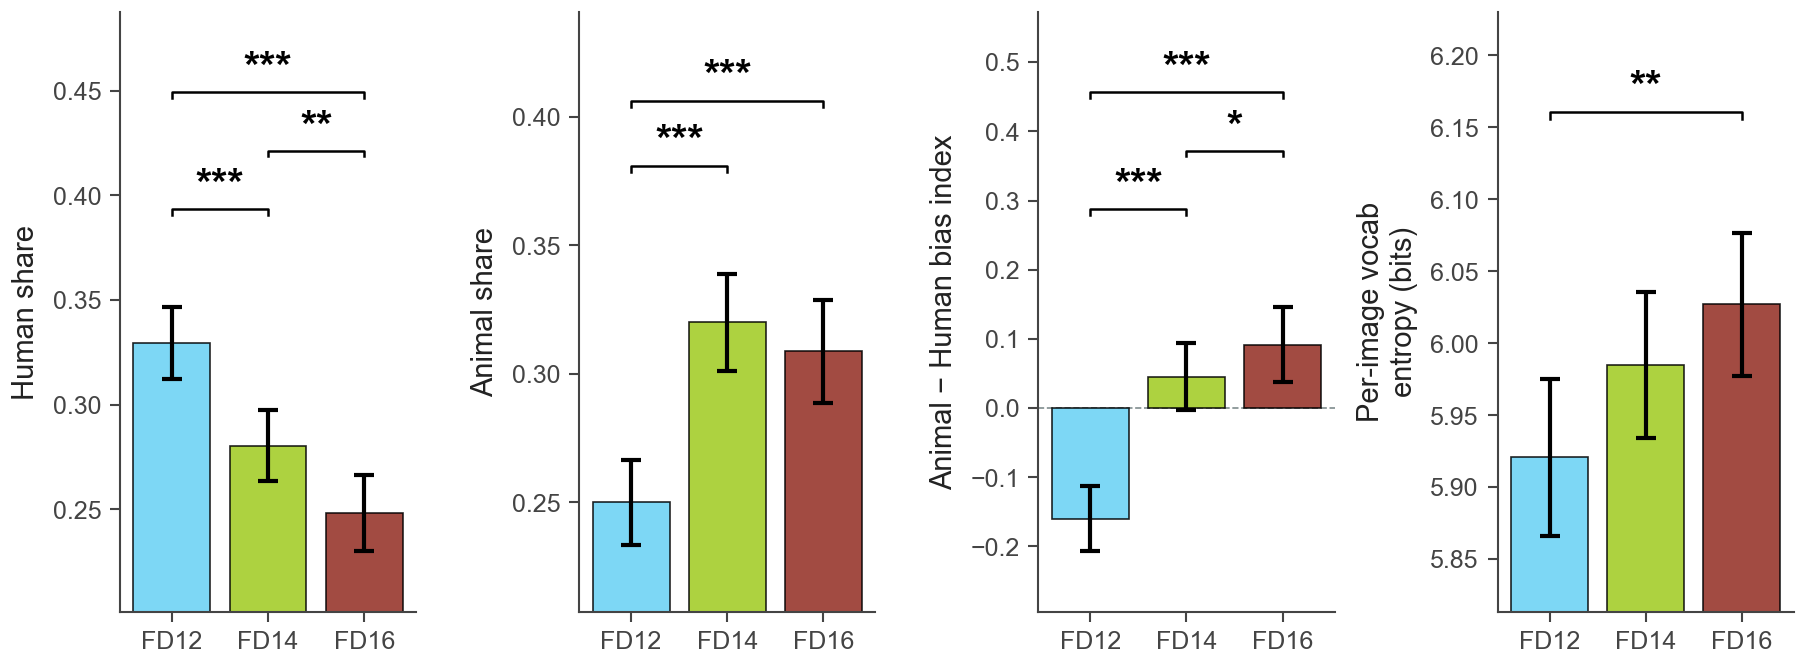
\includegraphics[width=\linewidth]{fig2_fd_perception.png}
\caption{\textbf{Image complexity reshapes the content of pareidolia.}
Within-subject mean $\pm$ 95\% CI per FD of the human share (face
$+$ body-part $+$ person), the animal share (mammal $+$ bird $+$ fish
$+$ insect), and the animal$-$human bias index $(A-H)/(A+H)$
(panels 1, 3), together with the per-image vocabulary entropy of
percept distributions (panel 4, violin = one distribution across the
ten images of each FD level). Brackets denote significant pair-wise
contrasts (Wilcoxon signed-rank for participant-level metrics,
Mann, Whitney U for the image-level violin). At low complexity (FD12)
percepts are dominated by discrete human-like figures; at intermediate
complexity (FD14) they shift toward animals; at high complexity (FD16)
they continue away from humans and inter-observer consensus declines.}
\label{fig:fd_perception}
\end{figure}

\begin{figure}[ht]
\centering
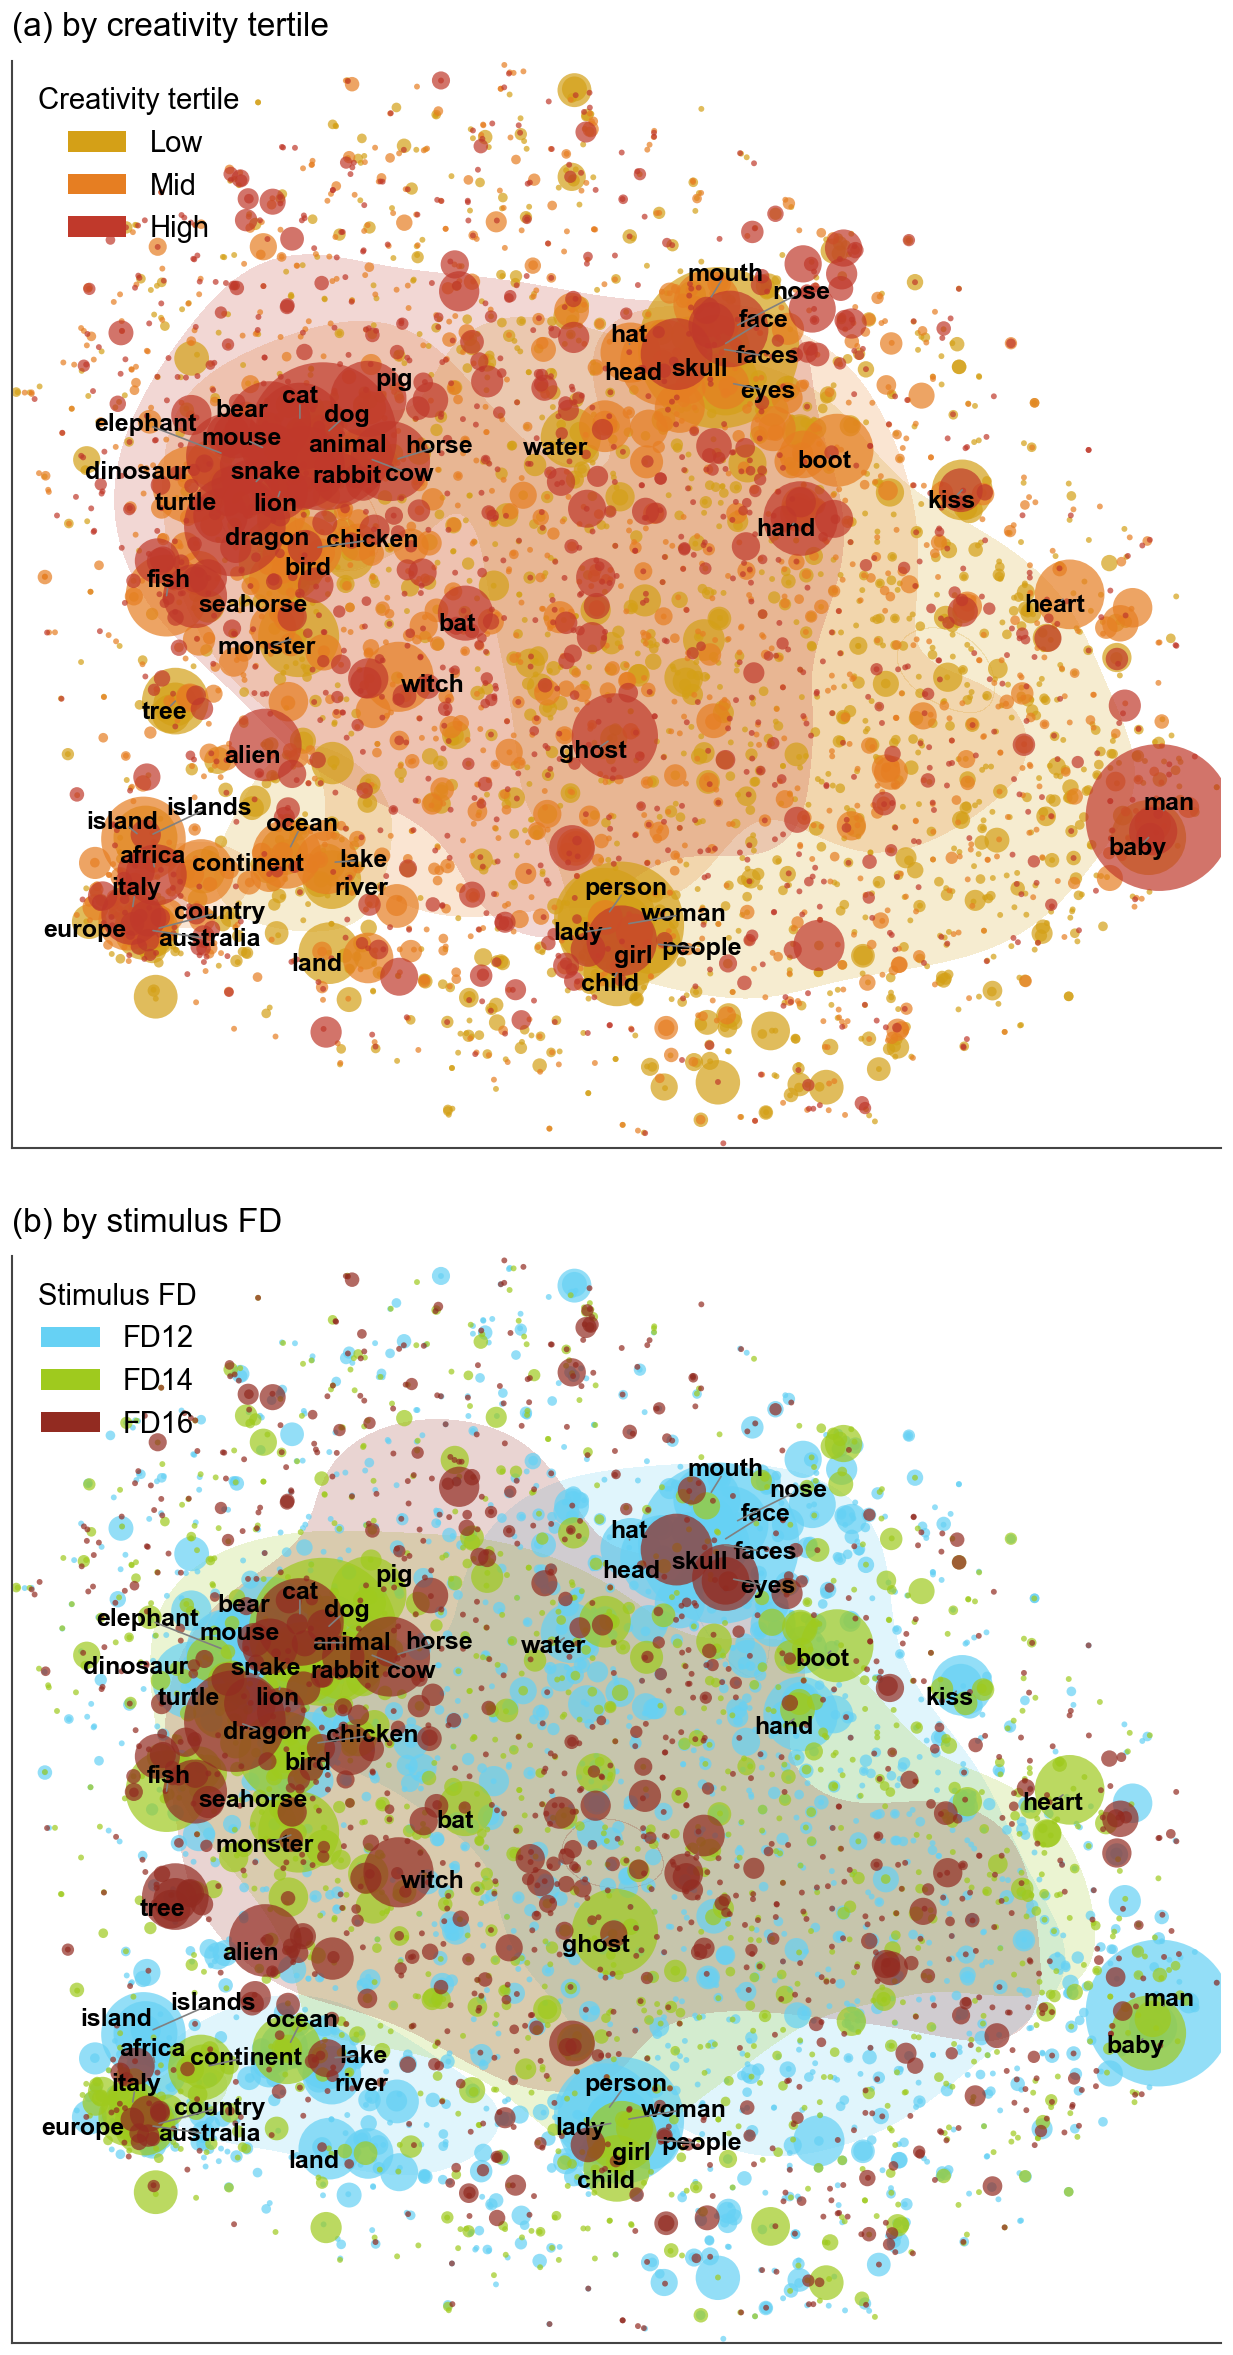
\includegraphics[width=0.78\linewidth]{fig3_semantic_territory.png}
\caption{\textbf{Semantic territory of collective pareidolia.} t-SNE
projection (cosine, perplexity~=~30) of every unique percept word
($n = 4{,}361$); dot size proportional to corpus frequency, KDE
contours per group. \textbf{(a)} colour by majority creativity tertile
of the speakers (sequential purple, light to dark = low to high DAT).
\textbf{(b)} colour by majority FD level at which the word was
produced. Both panels share the exact same projection.}
\label{fig:semantic_map}
\end{figure}

%, , , , , , , , , , , , , , , , , , , ,, 
\subsection{Trait creativity (DAT) effects}
\label{sec:dat}
%, , , , , , , , , , , , , , , , , , , ,, 

\paragraph{DAT-pre and DAT-post are correlated, but the link to
pareidolia lives at baseline.} Among the $n = 507$ participants who
completed both DAT timepoints (Fig.~\ref{fig:dat_pre_post}), pre- and
post-task scores were positively but moderately correlated (Pearson
$r = 0.19$, $p = 1.2 \times 10^{-5}$), with no detectable
group-level shift (Wilcoxon signed-rank $W = 6.1 \times 10^4$,
$p = 0.99$; mean $\Delta = -0.02$, SD $= 4.4$). The DAT, pareidolia
associations reported below replicate consistently with the pre-task
score and weaken substantially when the post-task score is
substituted in (data available in the supplementary tables),
consistent with the DAT, pareidolia link capturing a stable
trait-level property of the observer rather than a transient state
shift induced by completing the pareidolia task.

\begin{figure}[ht]
\centering
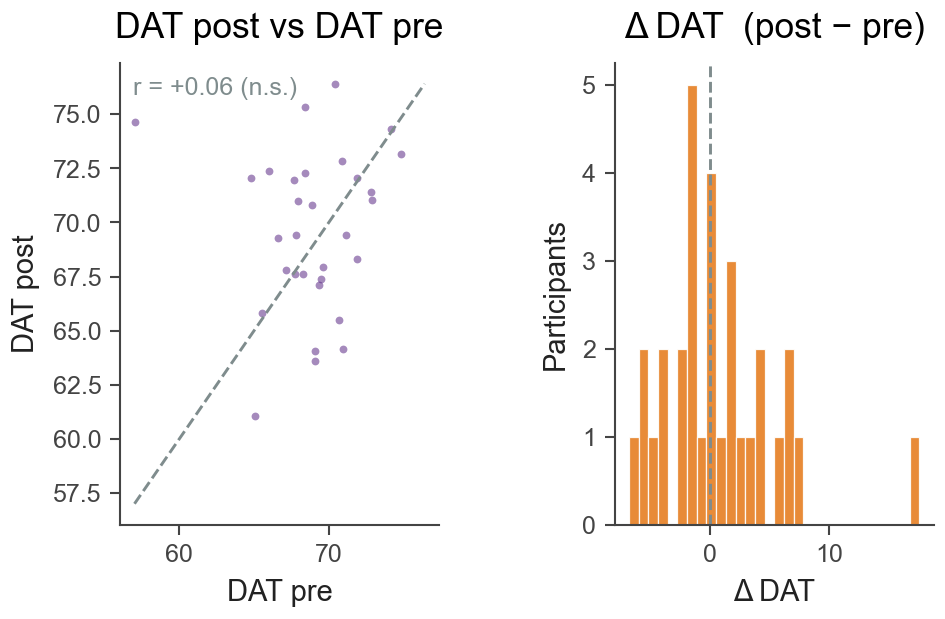
\includegraphics[width=0.85\linewidth]{fig5a_dat_pre_post.png}
\caption{\textbf{Pre vs post DAT scores.} Left: GloVe-scored DAT
post vs DAT pre, $n = 507$. Right: distribution of the participant-level
delta (post $-$ pre).}
\label{fig:dat_pre_post}
\end{figure}

\paragraph{Creativity is not associated with seeing more pareidolia.}
Across six general behavioural metrics, fraction of trials
completed, single words per trial, descriptions per trial, mean
reaction time, total unique words across the experiment, and mean
corpus rarity of a participant's words, only one survived bivariate
$\pm 3$~SD outlier trimming as significantly related to DAT, and in
the opposite direction to a ``more is more'' account: high-creativity
participants completed slightly \emph{fewer} trials than low-creativity
participants ($r = -0.10$, $p = 0.03$; Fig.~\ref{fig:dat_behaviour}).
Words per trial and reaction time were both null. Creativity, in this
dataset, therefore does not manifest as producing more or faster
pareidolia.

\begin{figure}[ht]
\centering
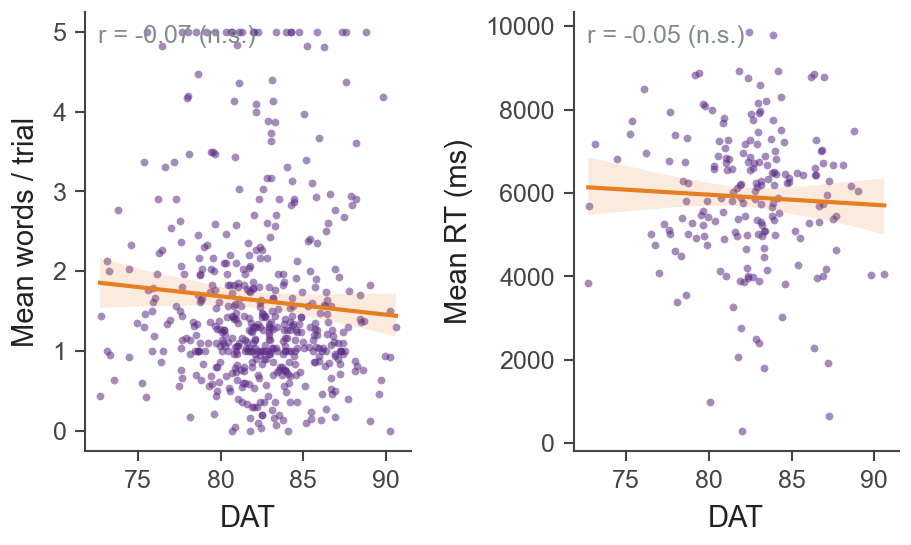
\includegraphics[width=\linewidth]{fig5b_dat_behaviour.png}
\caption{\textbf{Creativity and general pareidolia behaviour.} DAT vs
mean words per trial (left) and DAT vs mean reaction time (right).
Pearson $r$ and significance shown in-axis. The number of percepts
extracted per trial and the time taken to extract them do not
covary with creativity.}
\label{fig:dat_behaviour}
\end{figure}

\paragraph{Creativity predicts greater perceptual diversity, driven by
the middle complexity level.} The within-subject median pair-wise
cosine distance of a participant's percept embeddings, a
participant-level measure of how semantically scattered the percepts
they extract are, was positively correlated with DAT
($r = +0.14$, $p = 0.001$; $n = 500$; Fig.~\ref{fig:dat_diversity}),
reproducing a previously reported relationship between divergent
thinking and lexical diversity in a perceptual task. Splitting this
analysis by FD revealed that the effect is concentrated at the middle
complexity level (Fig.~\ref{fig:dat_diversity}b): $r = +0.17$
($p = 2.7 \times 10^{-4}$) at FD14, $r = +0.09$ ($p = 0.04$) at FD12,
and essentially null at FD16 ($r \approx 0$, $p = 0.93$).

\begin{figure}[ht]
\centering
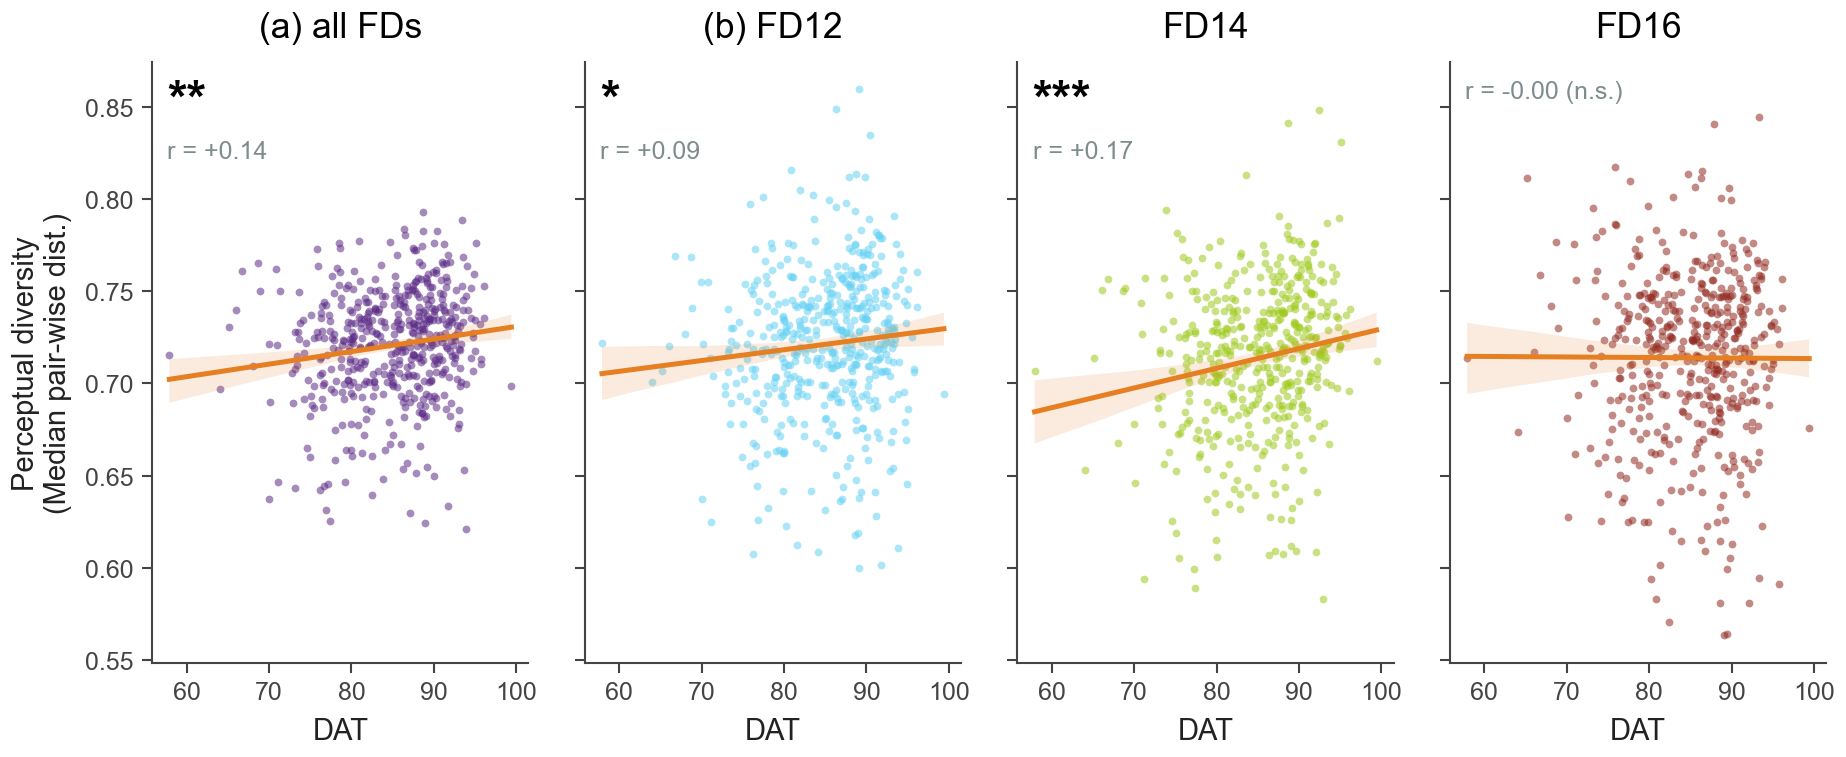
\includegraphics[width=\linewidth]{fig5cd_diversity.png}
\caption{\textbf{Creativity predicts perceptual diversity, especially
at the middle complexity level.} Within-subject median pair-wise
cosine distance of a participant's percept embeddings against DAT.
\textbf{(a)} pooled across all three FD levels (one point per
participant). \textbf{(b)} the same analysis split by FD: the
relationship is concentrated at FD14, the middle complexity level.}
\label{fig:dat_diversity}
\end{figure}

\paragraph{Creativity biases percepts away from humans and toward
animals.} A finer-grained category analysis pinpointed where the
DAT, diversity relationship comes from. The per-participant share of
percepts falling in human categories (face $+$ body-part $+$ person)
was negatively associated with DAT ($r = -0.12$, $p = 0.008$), while
the animal share was numerically higher in high-creativity
participants but did not reach significance on its own
($r = +0.07$, $p = 0.13$; Fig.~\ref{fig:dat_bias}). Combining the two
into an animal, human bias index produced the cleanest creativity
effect we observed ($r = +0.12$, $p = 0.010$; Spearman
$\rho = +0.13$, $p = 0.003$). High-creativity participants therefore
do not extract \emph{more} pareidolic percepts overall; rather, they
shift the \emph{kind} of percept they extract, away from canonical
human / face responses and toward animal-like ones.

\begin{figure}[ht]
\centering
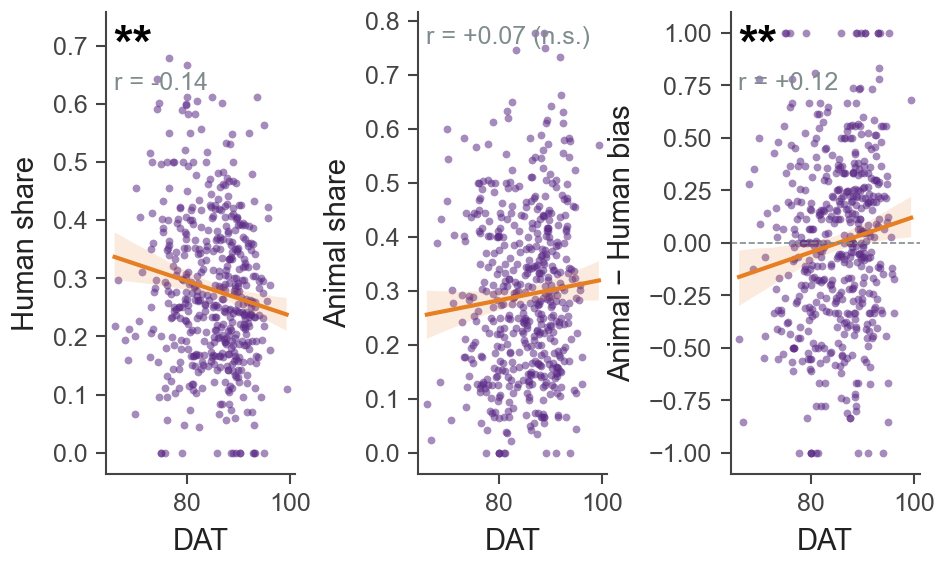
\includegraphics[width=\linewidth]{fig5f_dat_human_animal_bias.png}
\caption{\textbf{Creativity tilts the percept distribution away from
humans and toward animals.} Per-participant share of percepts that
fall in human categories (left), animal categories (centre), and the
animal-minus-human bias index (right) plotted against DAT. The
combined index gives the cleanest creativity effect.}
\label{fig:dat_bias}
\end{figure}

%, , , , , , , , , , , , , , , , , , , ,, 
\subsection{Data-driven percept clusters separate the two creativity
profiles}
%, , , , , , , , , , , , , , , , , , , ,, 

The human-vs-animal contrast captured one axis along which creativity
restructures percepts, but the seed-based taxonomy was deliberately
narrow. To examine the full preference landscape we re-derived
categories \emph{de novo} by clustering all percept words that occurred
at least three times in the corpus (Methods). HDBSCAN yielded 32
interpretable clusters plus a small noise group (22\% of words);
\(\sim\)$\frac{1}{3}$ of clusters had a 95\% bootstrap CI on the
log-odds (high vs low tertile) preference that excluded zero
(Fig.~\ref{fig:preferred_categories}b).

High-creativity participants were over-represented in clusters of
\emph{specific, embodied or unusual} percepts: \emph{mushroom / apple
/ clover / carrot}; \emph{gremlin / ogre / gargoyle / ghoul};
\emph{blood / stomach / kidney / vomit}; \emph{fish / seahorse / crab
/ whale}; \emph{bat / vase / ball / cob}; \emph{hand / finger / fist /
hands}; \emph{witch / cartoon / demon / angel}. Low-creativity
participants were over-represented in clusters of \emph{abstract or
texture-like} percepts: \emph{plus / separation / two / open};
\emph{water / spill / mess / pipe}; \emph{ink / paint / painting /
book}; \emph{ocean / lake / river / sea}; \emph{land / mountain /
cliff}; \emph{fire / explosion / death};
\emph{hammer / hole / splatter / dots}. The semantic-map view
(Fig.~\ref{fig:preferred_categories}a) makes the geographic structure
of the contrast explicit: the two preference profiles occupy
non-overlapping regions of BERT space, with the
``creature / viscera / specific-object'' region on the upper side and
the ``landscape / texture / abstract'' region on the lower side.
Together with the bias-index result above, this argues that the
creativity effect on pareidolia is best characterised not as
\emph{seeing more} but as \emph{seeing different things}.

\begin{figure}[ht]
\centering
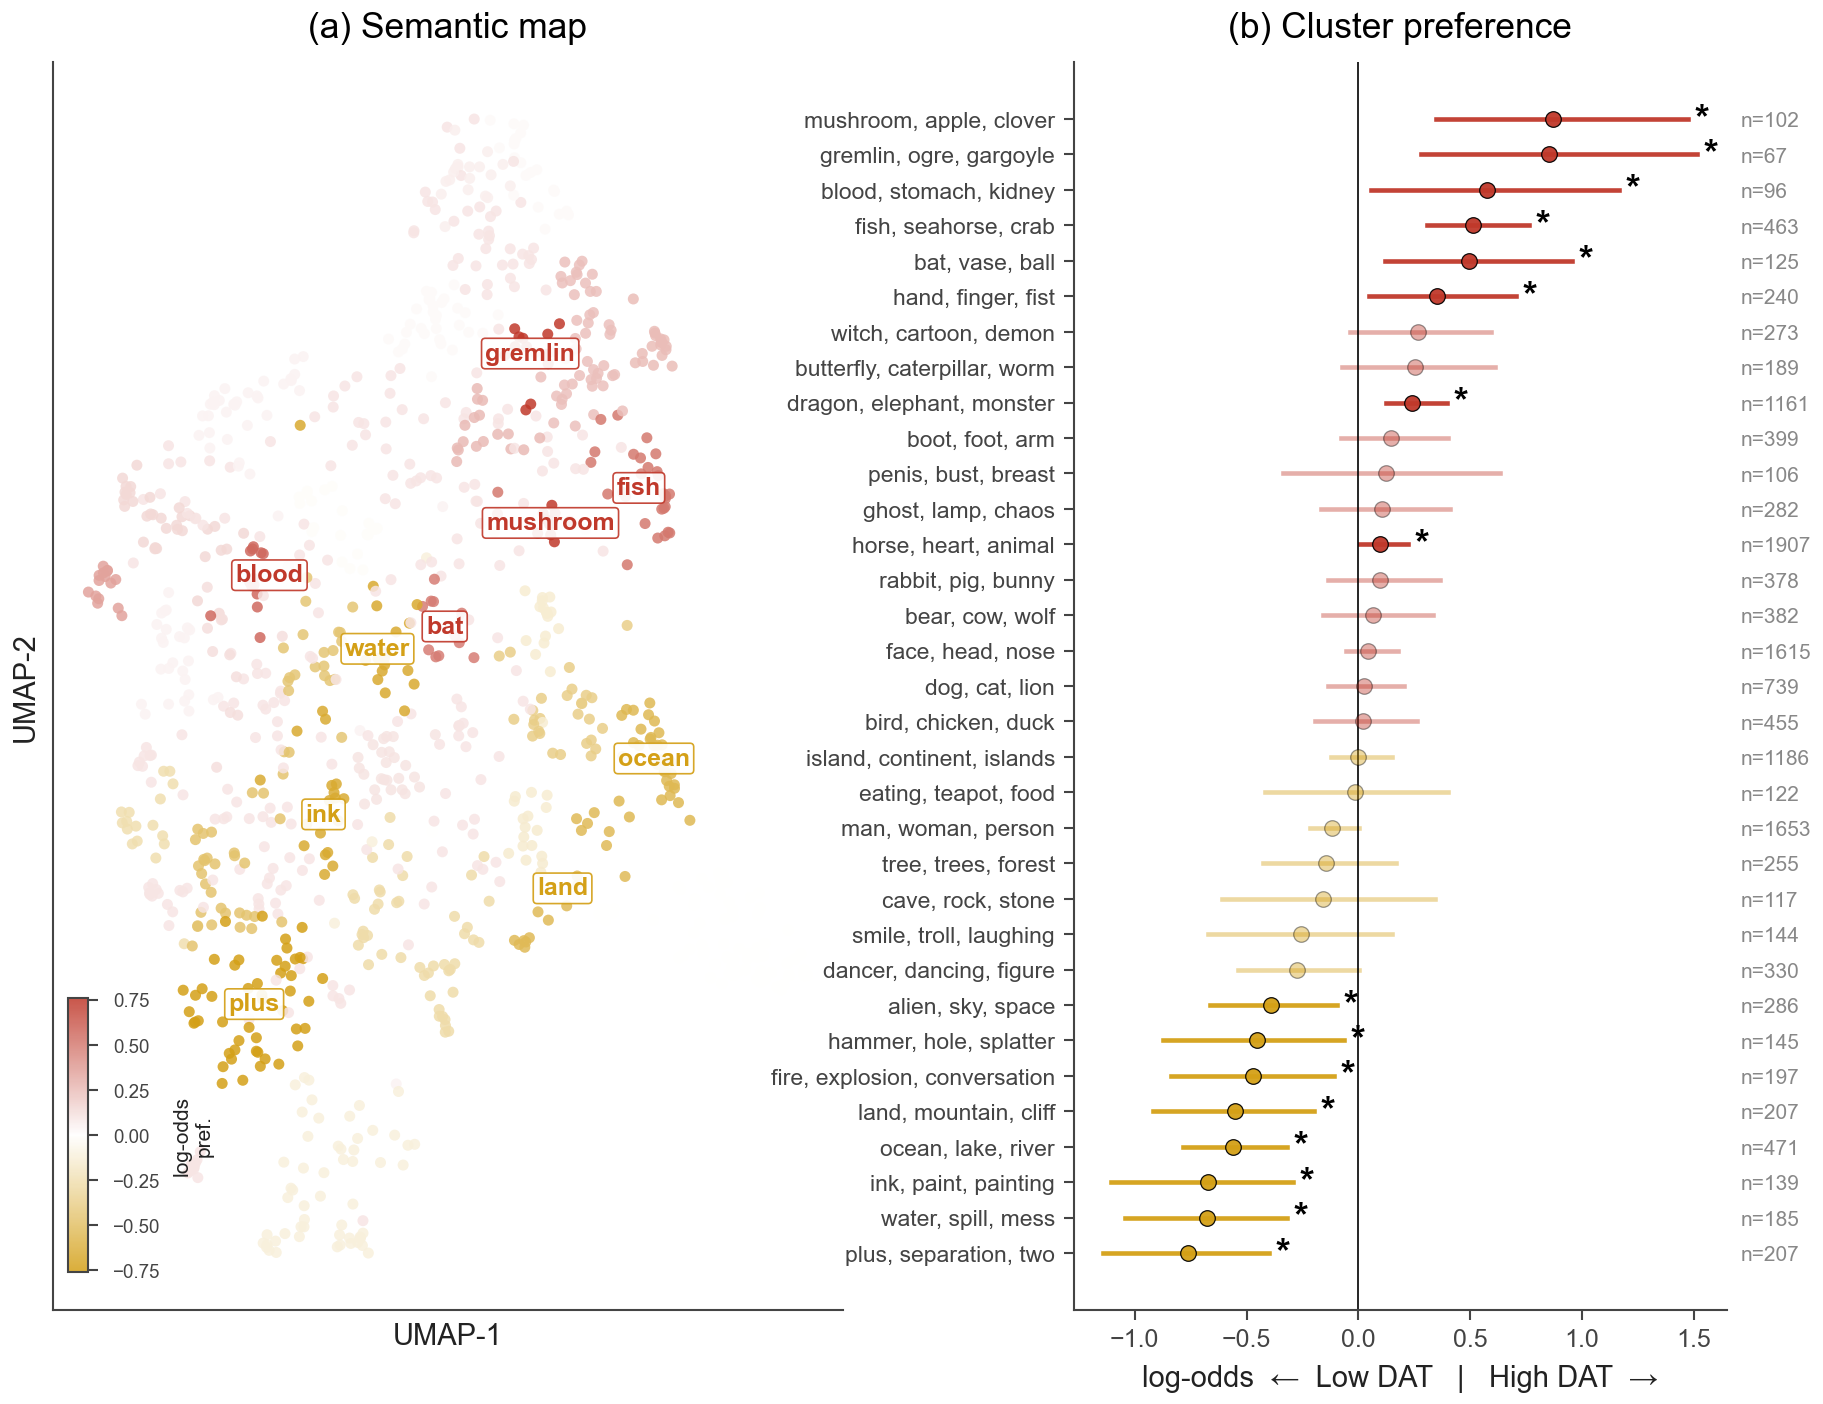
\includegraphics[width=\linewidth]{fig6_preferred_categories.png}
\caption{\textbf{Percept clusters preferred by low vs high creativity.}
\textbf{(a)} 2-D UMAP projection of every percept word with $\geq 3$
corpus occurrences, coloured by the log-odds preference of its HDBSCAN
cluster (red = preferred by high-creativity participants, blue =
preferred by low-creativity). Labels mark the top six clusters on each
side at their UMAP centroid. \textbf{(b)} Forest plot of all 32
retained clusters, log-odds (high$/$low) with bootstrap 95\% CI; stars
mark clusters whose CI excludes zero. Numbers in brackets are the word
occurrences per cluster.}
\label{fig:preferred_categories}
\end{figure}

The same clustering pipeline can be re-purposed with stimulus FD level
as the contrast variable (FD16 vs FD12 instead of high vs low DAT);
see Fig.~\ref{fig:preferred_categories_fd}. The FD contrast separates
an even larger set of clusters: high-FD images are over-represented
in clusters of \emph{tree / forest}, \emph{butterfly / caterpillar /
worm}, \emph{alien / sky / space}, \emph{fish / seahorse / crab},
\emph{witch / demon / angel} and \emph{ghost / lamp / chaos}, whereas
low-FD images dominate clusters of \emph{cave / rock / stones},
\emph{blood / stomach / kidney}, \emph{boot / foot / arm},
\emph{bat / vase / ball} and \emph{land / mountain / cliff}. The two
contrasts therefore highlight partly overlapping but distinct
preference geometries: creativity drives a humans-toward-animals shift
along one axis of BERT space, while stimulus complexity drives a
body-parts-toward-atmospheric-creatures shift along another.

\begin{figure}[ht]
\centering
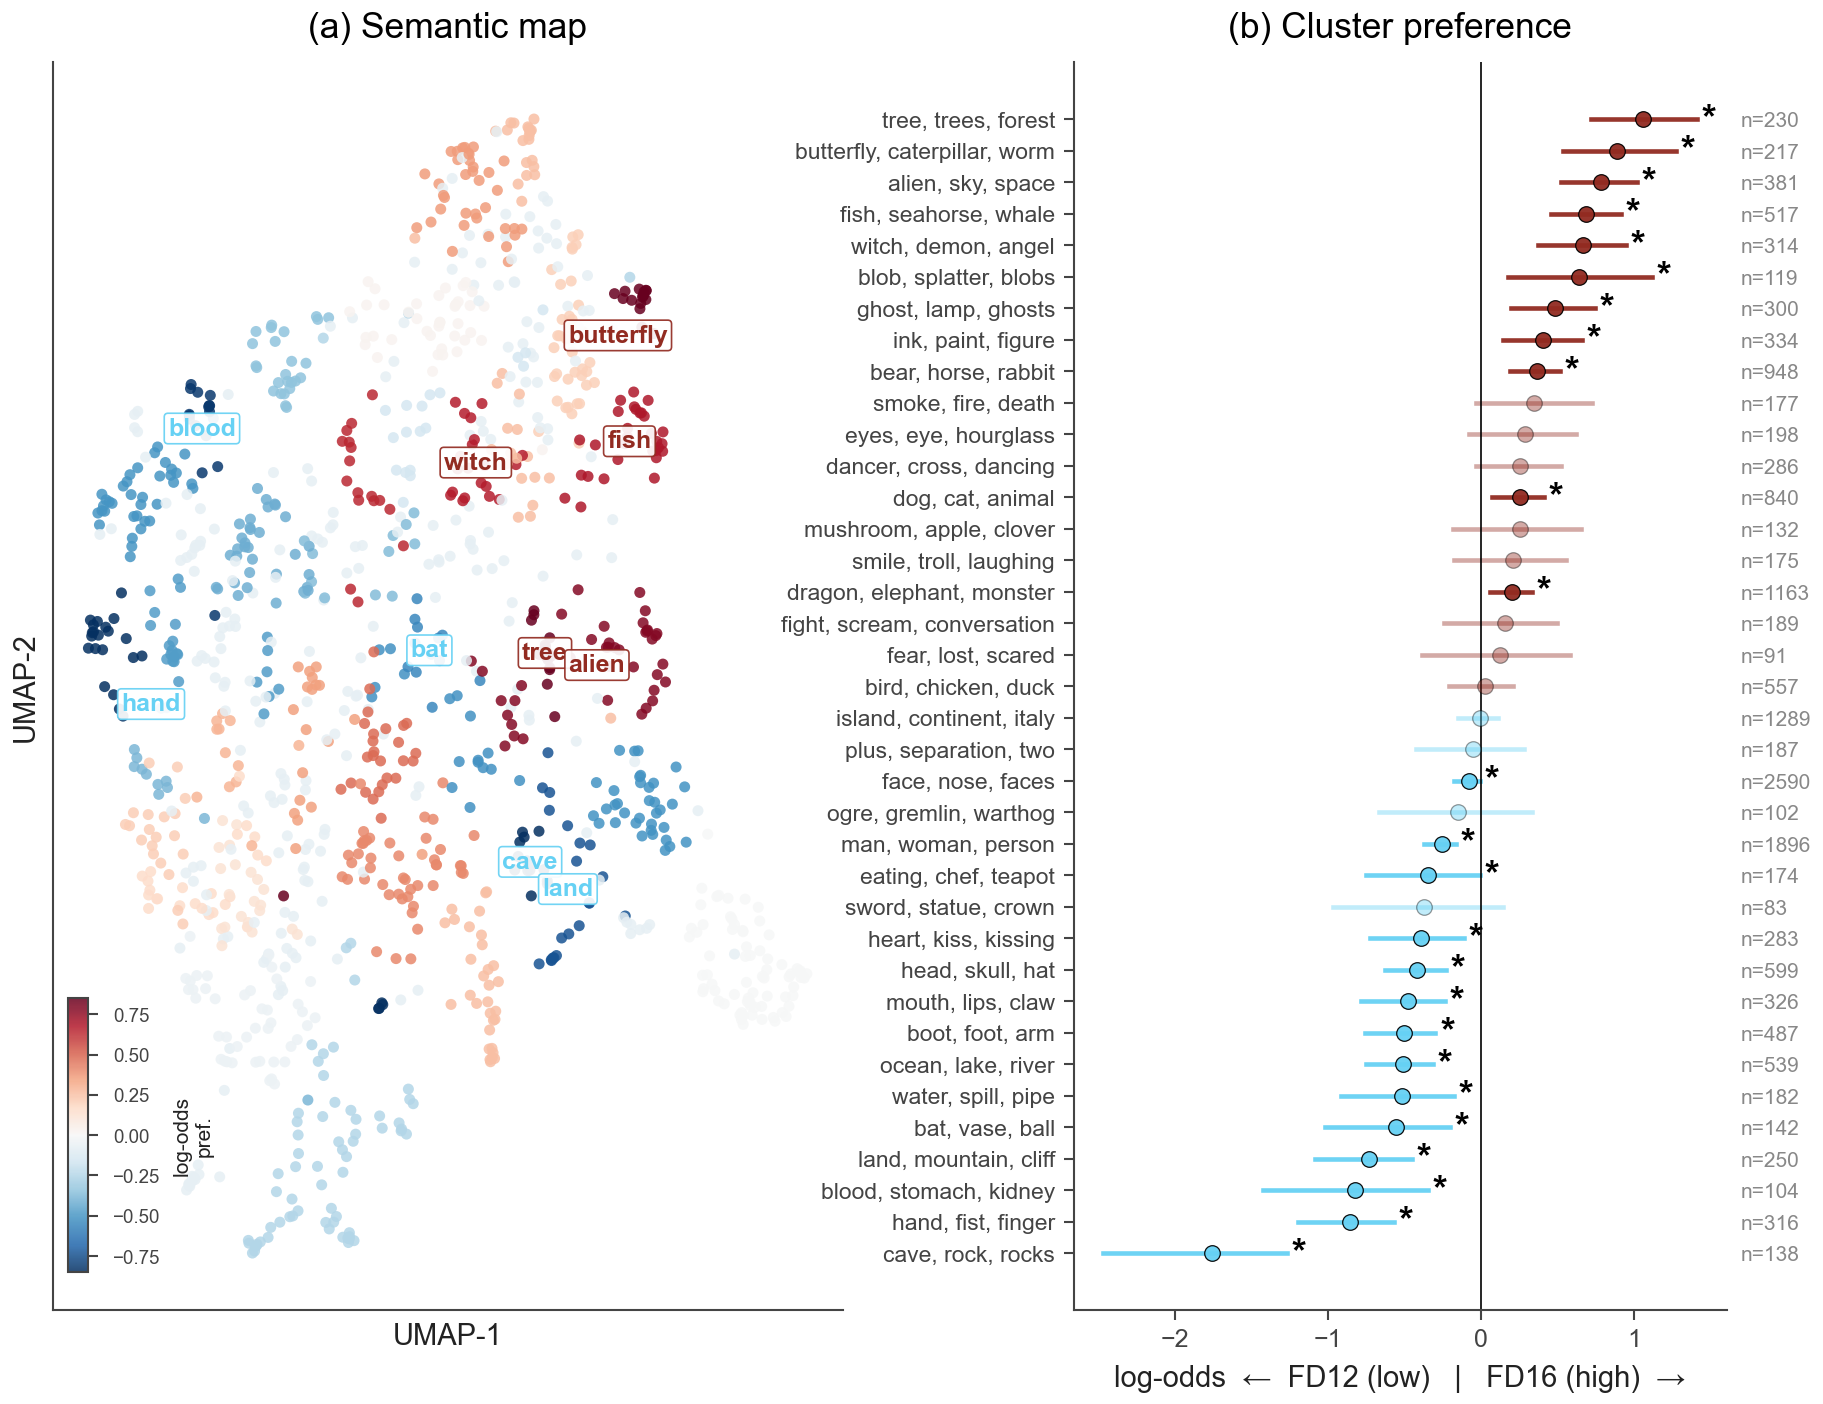
\includegraphics[width=\linewidth]{fig7_preferred_categories_fd.png}
\caption{\textbf{Percept clusters preferred by low vs high stimulus FD.}
Same clustering pipeline as Fig.~\ref{fig:preferred_categories}; the
contrast variable is FD16 versus FD12. \textbf{(a)} Semantic map
coloured by log-odds preference (blue = FD12, red = FD16).
\textbf{(b)} Forest plot of clusters, log-odds (FD16/FD12) with
bootstrap 95\% CI; stars mark clusters whose CI excludes zero.}
\label{fig:preferred_categories_fd}
\end{figure}

%==============================================================
\subsection{Eye tracking: a behavioural signature of successful pareidolia}

For the 247 participants who opted in to webcam-based gaze recording
and produced trials that survived the WebGazer tracking-failure check
(Methods), we computed six gaze metrics per trial spanning fixation
structure (count, mean duration), scanpath length, and three
spatial-concentration measures (gaze entropy in bits, Gini coefficient
of the 2-D gaze histogram, and recurrence rate of nearby fixations).
We contrasted these metrics along three independent axes: trials on
which the participant did vs did not report a pareidolic percept,
stimulus FD level, and continuous DAT score
(Fig.~\ref{fig:eye_tracking}).

\paragraph{Pareidolia trials are associated with more focused viewing.}
Within the 105 participants who had at least two trials of each kind,
trials in which the participant submitted at least one word
(``pareidolia'') differed from trials with no word (``no-pareidolia'')
on three of the six metrics, all in the same direction: more fixations
per trial (9.0 vs 9.4, Wilcoxon $p = 0.045$), lower 2-D gaze entropy
($3.76 \to 3.71$ bits, $p = 0.037$), and a higher Gini concentration
of the gaze distribution ($0.868 \to 0.872$, $p = 0.047$). Fixation
duration, scanpath length and recurrence rate did not differ.
Successful pareidolia is therefore accompanied by a small but
reliable shift toward \emph{more} fixations clustered in a
\emph{smaller} region, consistent with the participant having found
something specific in the noise that they are inspecting.

\paragraph{Stimulus complexity reshapes the scan pattern.}
Within-subject FD effects emerged on scanpath length (Friedman
$p = 0.006$; FD12 $\to$ FD16 monotonic decrease) and, marginally, on
fixation duration (Friedman $p = 0.06$; longer fixations at FD16).
The other four metrics were not modulated by FD. The pattern
suggests that as image complexity rises, participants move their eyes
less and dwell on a few central locations for longer, consistent with
the behavioural and content-level FD effects in
Figs.~\ref{fig:fd_behaviour} and \ref{fig:fd_perception}.

\paragraph{Eye movements are not predicted by trait creativity.}
None of the six metrics correlated reliably with DAT score
($|r| < 0.07$ for all six; all $p > 0.30$). Together with the
behavioural-engagement null in Sec.~\ref{sec:dat}, this argues that
creativity does not change \emph{how} people look at the stimulus,
only \emph{what} they extract from it.

\begin{figure}[ht]
\centering
\includegraphics[width=\linewidth]{fig4_eye_tracking.png}
\caption{\textbf{Eye-tracking metrics across three contrasts.}
Rows: (A) pareidolia vs no-pareidolia trials (within-subject
Wilcoxon, $n = 105$ participants with $\geq 2$ trials of each kind);
(B) stimulus FD level (within-subject Friedman + pair-wise Wilcoxon,
$n = 226$); (C) continuous DAT score (between-subject Pearson,
$n = 198$--$227$ depending on the metric, $\pm 3$ SD bivariate trim).
Columns: six gaze metrics, mixing classical (fixation count, fixation
duration, scanpath length, gaze entropy) and recent measures (Gini
concentration of the 2-D gaze histogram, RQA-style recurrence rate of
nearby fixations). Brackets mark significant pair-wise contrasts;
small in-axis text on row C reports Pearson $r$.}
\label{fig:eye_tracking}
\end{figure}


\bibliographystyle{plainnat}
\begin{thebibliography}{1}
\bibitem[Olson et~al.(2021)]{Olson2021dat}
J.~A. Olson, J.~Nahas, D.~Chmoulevitch, S.~J. Cropper, and M.~E. Webb.
\newblock Naming unrelated words predicts creativity.
\newblock {\em Proceedings of the National Academy of Sciences},
118(25):e2022340118, 2021.
\end{thebibliography}

\end{document}
